\section{Machine Learning Modeling}

This section delves into the systematic process of developing, training and evaluating algorithms, which empower data-driven learning, predictions, and decisions. This process encompasses selecting an appropriate algorithm, designing the model architecture, preprocessing and transforming data, and extracting relevant features. By iteratively adjusting the model's parameters, we aim to minimize the prediction error. The choice of techniques, such as supervised, unsupervised, or reinforcement learning, is dictated by the specific problem and data structure. Model evaluation, fine-tuning, and deployment are essential to ensure the model generalizes well to new data and performs effectively in real-world applications.

\def\circRad{4em}

\begin{figure}
    \centering
    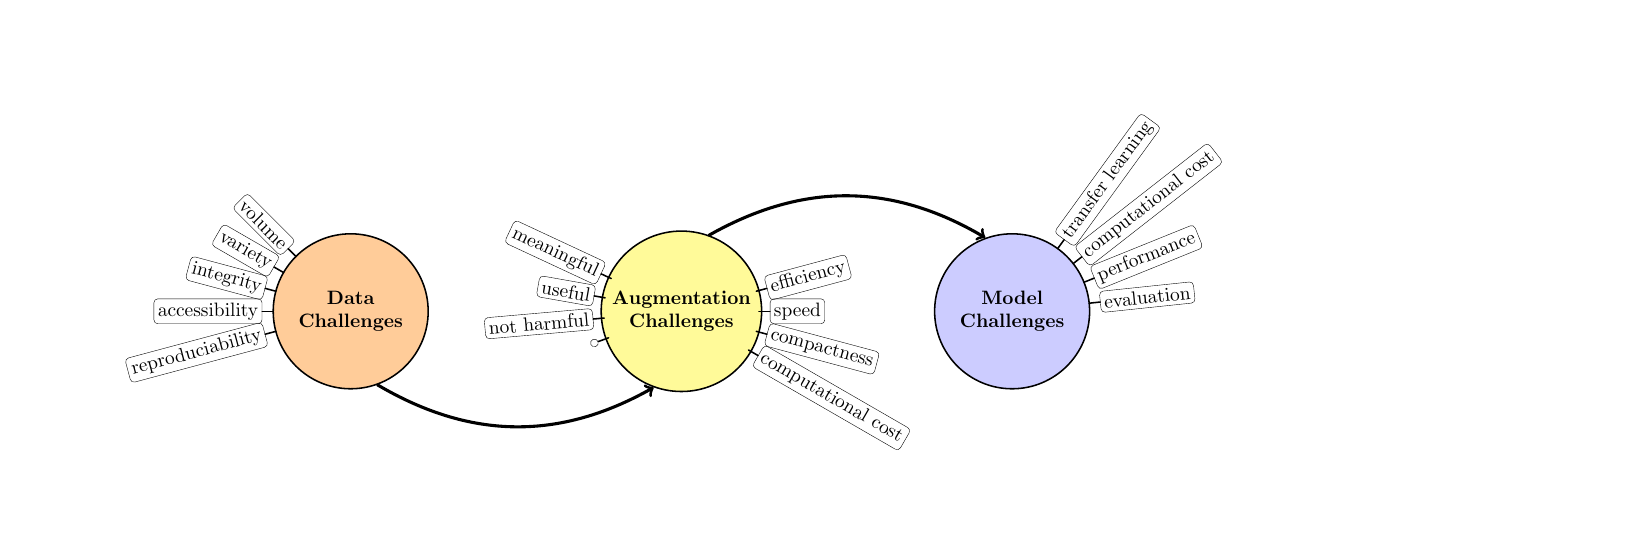
\begin{tikzpicture}[
    line cap=round, thick,
    stage/.style={shape=circle, draw, font=\bfseries, minimum width=2*\circRad},
    challenge/.style={draw, very thin, inner sep=2, rounded corners=2},
    every node/.style={align=center},
  ]
\centering
\scalebox{0.7}{
  \begin{scope}[local bounding box=challenges]
    % Data
    \node [stage, fill=orange!40] (data) {Data\\Challenges};
    \foreach \itm [count=\i, evaluate={\a=\i*15+120;}] in
      {volume, variety, integrity, accessibility, reproduciability} {
        \node[challenge] at (\a:\circRad + 2mm) [rotate=\a+180, anchor=east] {\itm};
        \draw (\a:\circRad + 2mm) -- (\a:\circRad);
      }

    % Transformations
    \begin{scope}[xshift=6cm]
      \node [stage, fill=yellow!40] (descriptor) {Augmentation\\Challenges};
      \foreach \itm [count=\i, evaluate={\a=\i*15+140;}] in
        {meaningful, useful, not harmful,} {
          \node[challenge] at (\a:\circRad + 2mm) [rotate=\a+180, anchor=east] {\itm};
          \draw (\a:\circRad + 2mm) -- (\a:\circRad);
        }
      \foreach \itm [count=\i, evaluate={\a=30-\i*15;}] in
        {efficiency, speed, compactness, computational cost} {
          \node[challenge] at (\a:\circRad + 2mm) [rotate=\a, anchor=west] {\itm};
          \draw (\a:\circRad + 2mm) -- (\a:\circRad);
        }
    \end{scope}

    % Model
    \begin{scope}[xshift=12cm]
      \node [stage, fill=blue!20] (model) {Model\\Challenges};
      \foreach \itm [count=\i, evaluate={\a=70-\i*16;}] in
        {transfer learning, computational cost, performance, evaluation} {
          \node[challenge] at (\a:\circRad + 2mm) [rotate=\a, anchor=west] {\itm};
          \draw (\a:\circRad + 2mm) -- (\a:\circRad);
        }
    \end{scope}
  \end{scope}

  \draw[ultra thick,->] (data.-70) to [bend right] (descriptor.-110);
  \draw[ultra thick,->] (descriptor.70) to [bend left] (model.110);
    }
\end{tikzpicture}
    \caption[Challenges in Data, Augmentation, and Model Stages]{\small{A visual representation of the challenges in three main stages of a machine learning pipeline: Data, Augmentation, and Model. The Data stage includes challenges such as volume, variety, integrity, accessibility, and reproducibility. The Augmentation stage covers challenges related to creating meaningful, useful, and not harmful augmentations while considering efficiency, speed, compactness, and computational cost. The Model stage addresses challenges in transfer learning, computational cost, performance, and evaluation. Arrows indicate the flow of progression from one stage to another.}}

    \label{fig:my_label}
\end{figure}


\subsection{Model architecture and training strategy}

Given the nature of our task, we propose using a Triple Siamese Network. This model architecture has been proven efficient for music similarity retrieval tasks \cite{contentmusicsimtriplet2020}. Specifically, we aim to minimize the loss function between an anchor, a positive, and a negative sample by using online triplet mining \cite{Sikaroudi2020OfflinePatches}.

Using the proposed triple siamese network and online triplet mining, we aim to train a model that can effectively distinguish between similar and dissimilar samples while considering their underlying composition and production texture.

\subsection{Problem to solve}

\subsection{Self-Supervised Learning (SSL)}

Self-supervised learning (SSL) is a subfield of machine learning where models learn to generate representations of data by finding patterns and structures within the data without relying on external labels or annotations. In other words, the model learns by creating its supervision signal from the raw, unlabeled data.\cite{audioselfsupsurvey}

This approach to learning is inspired by the way humans and animals learn from their environment, where a great deal of knowledge is acquired through observation and interaction without explicit instruction. SSL algorithms often involve tasks where the model learns to predict or reconstruct parts of the input data, such as predicting the next word in a sentence or completing an image with missing pixels.

Some of the main advantages of SSL include:

\begin{enumerate}
\item Reduces dependency on labeled data, which can be expensive and time-consuming to collect and annotate.
\item Encourages more generalizable and robust representations of the data since they capture the inherent structure and properties of the data rather than relying on human-provided labels.
\end{enumerate}

\subsubsection{Known and unknown invariance}

This section discusses the concepts of known and unknown invariance in pattern recognition. Invariance refers to the property of a model or algorithm being robust to certain transformations or changes in the input data. In other words, an invariant model should produce the same or similar output for different instances of the same object, even if they have undergone some changes.

Known invariance: Known invariances are transformations or changes that the model or algorithm is explicitly designed to be robust against. This can include the input data's rotations, translations, scaling, or other known perturbations. By incorporating these invariances into the model's design, the algorithm is better equipped to generalize and recognize patterns in the presence of these transformations.

Unknown invariance: Unknown invariances are transformations or changes the model has not been explicitly designed to handle. However, it still manages to be robust due to its learning capabilities. These invariances can emerge from the data and may not be known a priori. For example, a deep learning model might automatically learn to be invariant to certain lighting conditions or other factors not explicitly specified in its design.

\begin{equation}
\label{eq:invariance_to_particular_transformation_function}
\forall x \in X, \forall y \in Y, \forall \rho \in \mathcal{T}, f(x) = f(y) \implies f(\rho(x)) = f(\rho(y))
\end{equation}

In expression \ref{eq:invariance_to_particular_transformation_function}, $X$ and $Y$ represent sets of input data, $\rho$ represents a transformation function, and $f$ represents a machine learning model. The expression states that for all inputs $x$ and $y$ in $X$ and $Y$, if $f(x) = f(y)$, then $f(\rho(x)) = f(\rho(y))$.

The expression specifies that a model is invariant to a particular transformation function $\rho$ if it produces the same output for both the original and transformed input.

\subsection{Contrastive Learning of Musical Representations (CLMR)}

Contrastive Learning of Musical Representations (CLMR) \cite{CLMR2021} aims to learn discriminative and valuable representations of music without relying on explicit labels. By leveraging the structure and content of music and contrasting different augmentations or transformations of the same musical piece against randomly generated pieces, CLMR models can effectively capture the underlying known invariances that are explicitly incorporated into the design of a model to improve its robustness and generalization.

In contrast, the model learns unknown invariances from the data without explicit instruction.

The CLMR methodology involves the following steps:

\begin{enumerate}
\item \textbf{Data Augmentation:} Create different augmentations or transformations of the same musical piece as positive pairs and use other randomly selected pieces as antagonistic pairs.
\item \textbf{Contrastive Learning:} Train by minimizing a contrastive loss function, encouraging the model to produce similar representations for positive pairs and dissimilar representations for antagonistic pairs.
\item\textbf{Latent Representation:} Utilize the learned representations for various Music Information Retrieval (MIR) downstream tasks, such as music genre classification or similarity, both in the symbolic and time domains.
\end{enumerate}

By following these steps, CLMR models can learn meaningful and robust representations of music, potentially enhancing their performance in various MIR tasks and reducing the need for labeled data.

\subsection{Siamese Networks}

A Siamese Network, a deep learning architecture introduced by Bromley and LeCun in the early 1990s \cite{Bromley1993SignatureNetwork}, is designed explicitly for tasks involving similarity or comparison between two input instances, such as signature verification. Its name derives from the structure, which consists of two or more identical subnetworks connected in parallel and joined at the output layer. These subnetworks share the same architecture, weights, and hyperparameters, allowing for more efficient memory usage and computational complexity. This design is particularly effective for learning from limited or imbalanced datasets, as it focuses on learning the similarity metric rather than specific features of individual classes.

Each subnetwork processes an input independently, and its outputs are combined and further processed to yield a single similarity score. The shared weights during training enable the model to learn an invariant representation for the input instances, improving its efficiency in comparing and contrasting them. Siamese Networks employ specialized loss functions, such as contrastive or triplet loss, which minimize the distance between similar input pairs and maximize the distance between dissimilar ones. This approach encourages the network to learn a meaningful similarity metric.


\subsection{Triplet Siamese Networks}


Triplet Siamese Networks, an extension of the Siamese Network architecture, involve comparing three input instances instead of two, aiming to learn an embedding space where similar instances are close and dissimilar instances are distant. The input consists of an anchor, a positive instance (same class as the anchor), and a negative instance (different class). Each instance is processed by an identical subnetwork with shared architecture, weights, and hyperparameters.

The triplet loss function guides learning, minimizing the distance between the anchor and positive instances while maximizing the distance between the anchor and negative instances. A margin parameter in the loss function ensures a minimum separation between positive and negative instances in the embedding space.

Triplet Siamese Networks offer several advantages, including learning fine-grained similarity metrics, being well-suited for one-shot learning tasks, and offering efficient memory usage and computational complexity due to shared weights. These networks have been applied to various tasks and domains, such as image recognition, face recognition, speaker recognition, text similarity, and medical imaging for diagnosis or treatment purposes.

\subsection{XXX}
\subsection{XXX}

\subsection{Encoder}
\subsubsection{SampleCNN}

The SampleCNN model \cite{CLMR2021} takes in 1D input data with a single channel. The first layer is a 1D convolutional layer with a kernel size of 3, a stride of 3, and 128 output channels. It is followed by batch normalization and ReLU activation.

After the initial layer, there are nine hidden layers with varying kernel sizes, strides, and channels. Each hidden layer consists of the following:

\begin{itemize}
    \item A 1D convolutional layer with the specified number of input and output channels, kernel size, a stride of 1, and padding of 1.

    \begin{equation}
y_{c_o}(n) = \sum_{c_i=1}^{C_{\text{in}}} \sum_{k=-\lfloor K/2 \rfloor}^{\lfloor K/2 \rfloor} x_{c_i}(n - k) \cdot w_{c_o, c_i}(k)
\end{equation}

Where:

$y_{c_o}(n)$ is the output for the $c_o$-th output channel at position $n$
$C_{\text{in}}$ is the number of input channels
$x_{c_i}(n)$ is the input for the $c_i$-th input channel at position $n$
$w_{c_o, c_i}(k)$ is the kernel weight for the $c_o$-th output channel and $c_i$-th input channel at position $k$
$K$ is the kernel size
The stride is set to 1, and padding is set to 1 (equal padding $\lfloor K/2 \rfloor$ on both sides)
s
    \item Batch normalization. We process a batch of data containing anchor, positive, and negative samples. We pad the waveforms to the same  maximum length among the collection, perform online triplet mining to find the hardest negatives and return the padded anchors, positives, and hardest negatives.

    Let $A$, $P$, and $N$ represent the anchor, positive, and negative samples. The maximum array length in the batch is given by:

    \begin{equation}
L_{\text{max}} = \max_{\text{item} \in \text{batch}}(\max(\text{length}(A_{\text{item}}), \text{length}(P_{\text{item}}), \text{length}(N_{\text{item}})))
\end{equation}

    The anchor-positive distance and the anchor-negative distance are computed as the Euclidean distance between the corresponding samples:

    \begin{equation}
D_{\text{AP}} = \sqrt{\sum_{i} (A_i - P_i)^2}
\end{equation}

    The "hardest" negative index for each anchor-positive pair is determined by maximizing the difference between the anchor-negative and anchor-positive distances:

    \begin{equation}
D_{\text{AN}} = \sqrt{\sum_{i} (A_i - N_i)^2}
\end{equation}

    
    \item ReLU activation. The Rectified Linear Unit (ReLU) activation function is a simple yet highly effective non-linear function used in neural networks. It helps introduce non-linearity to the model and accelerates training due to its computational efficiency.

    
    \item Max pooling with kernel size and stride equal to the stride value of the current layer.
\end{itemize}

\begin{tabular}{|c|c|c|}
\hline
\textbf{Layer} & \textbf{Input Channels} & \textbf{Output Channels} \\
\hline
1 & 128 & 128 \\
\hline
2 & 128 & 128 \\
\hline
3 & 128 & 256 \\
\hline
4 & 256 & 256 \\
\hline
5 & 256 & 256 \\
\hline
6 & 256 & 256 \\
\hline
7 & 256 & 256 \\
\hline
8 & 256 & 256 \\
\hline
9 & 256 & 512 \\
\hline
\end{tabular}

After the hidden layers, there's another 1D convolutional layer with 512 input channels, 512 output channels, a kernel size of 3, a stride of 1, and padding of 1. This is followed by batch normalization and ReLU activation.

The output of the final convolutional layer is passed through an average pooling operation across the temporal dimension (dim=2).

If the model is "supervised", dropout with a rate of 0.5 is applied; a regularization technique randomly drops out neurons during training to prevent overfitting, with a 0.5 rate meaning half of the neurons are dropped out.

\def\layersep{2}
\def\nodesep{1.5}

\begin{figure}[h]
    \centering
    \scalebox{0.7}{
    \begin{tikzpicture}[node/.style={circle, draw, thick}]
  % TikZ code here
  \foreach \y in {1,...,5}{
      \node[node] (i\y) at (0,\nodesep*\y) {};
      \node[node, right=\layersep of i\y] (h1\y) {};
      \node[node, right=\layersep of h1\y] (h2\y) {};
    }

  \node[node, right=\layersep of h22] (o1) {};
  \node[node, right=\layersep of h24] (o2) {};

  \foreach \source in {1,...,5}
  \foreach \dest in {1,...,5}{
      \path[-stealth, thick] (i\source) edge (h1\dest);
      \path[-stealth, thick] (h1\source) edge (h2\dest);
    }
  \foreach \source in {1,...,5}
  \foreach \dest in {1,2}
  \draw[-stealth, thick] (h2\source) -- (o\dest);

  \draw[-stealth, thick] (8.3,3*\nodesep) -- node[above,font=\Large\bfseries] {dropout} (10.3, 3*\nodesep);

  % Boundary

  \foreach \y in {1,...,5}
  \node[node, right=15em of h2\y] (di\y) {};

  \node[red,font=\huge] at (di1) {$\times$};
  \node[red,font=\huge] at (di3) {$\times$};

  \foreach \y in {1,...,5}
  \node[node, right=\layersep of di\y] (dh1\y) {};

  \node[red,font=\huge] at (dh11) {$\times$};
  \node[red,font=\huge] at (dh13) {$\times$};
  \node[red,font=\huge] at (dh14) {$\times$};

  \foreach \y in {1,...,5}
  \node[node, right=\layersep of dh1\y] (dh2\y) {};

  \node[red,font=\huge] at (dh22) {$\times$};
  \node[red,font=\huge] at (dh24) {$\times$};

  \node[node, right=\layersep of dh22] (do1) {};
  \node[node, right=\layersep of dh24] (do2) {};

  \foreach \source in {2,4,5}
  \foreach \dest in {2,5}
  \draw[-stealth, thick] (di\source) -- (dh1\dest);

  \foreach \source in {2,5}
  \foreach \dest in {1,3,5}
  \draw[-stealth, thick] (dh1\source) -- (dh2\dest);

  \foreach \source in {1,3,5}
  \foreach \dest in {1,2}
  \draw[-stealth, thick] (dh2\source) -- (do\dest);

\end{tikzpicture}
    }
    \caption{\small{High-level schematic dropout representation}}
    \label{figure: dropout}
\end{figure}

Finally, a linear layer with 512 input features and 128 output dimension features is applied to generate the embeddings.

\begin{tikzpicture}[
  node distance=0.5cm,
  block/.style={draw, rectangle, fill=blue!20, text width=1.5cm, align=center, minimum height=1cm},
  arrow/.style={->, >=stealth, line width=0.5mm}
]

% Input
\node (input) [block] {Input};

% Conv 1
\node (conv1) [block, right=of input] {Conv1D\\128};
\draw[arrow] (input) -- (conv1);

% BatchNorm 1 and ReLU 1
\node (bn1) [block, right=of conv1] {BatchNorm\\ReLU};
\draw[arrow] (conv1) -- (bn1);

% Hidden Layers
\node (hidden1) [block, right=of bn1] {Hidden Layer 1};
\draw[arrow] (bn1) -- (hidden1);

\node (hidden2) [block, right=of hidden1] {Hidden Layer 2};
\draw[arrow] (hidden1) -- (hidden2);

\node (hidden3) [block, right=of hidden2] {Hidden Layer 3};
\draw[arrow] (hidden2) -- (hidden3);

\node (dots) [right=of hidden3] {$\cdots$};
\draw[arrow] (hidden3) -- (dots);

% Conv N
\node (convN) [block, right=of dots] {Conv1D\\512};
\draw[arrow] (dots) -- (convN);

% BatchNorm N and ReLU N
\node (bnN) [block, right=of convN] {BatchNorm\\ReLU};
\draw[arrow] (convN) -- (bnN);

% Average Pooling
\node (avgpool) [block, right=of bnN] {Avg Pool};
\draw[arrow] (bnN) -- (avgpool);

% Dropout (optional)
\node (dropout) [block, right=of avgpool, dashed] {Dropout (optional)};
\draw[arrow, dashed] (avgpool) -- (dropout);

% Fully Connected
\node (fc) [block, right=of dropout] {Linear\\Out\_dim};
\draw[arrow] (dropout) -- (fc);

\end{tikzpicture}


We have adapted the original architecture for our experiments to our purpose, which consists of the final average pooling step.

\begin{equation}
y_i = \frac{1}{N} \sum_{j=1}^{N} x_{ij}
\end{equation}

\begin{itemize}
  \item \(y_i\) represents the output tensor after the average pooling operation,
  \item \(x_{ij}\) represents the elements in the 2D input tensor,
  \item \(N\) is the number of elements along the second dimension of the input tensor,
  \item \(i\) iterates over the first dimension of the tensors, and
  \item \(j\) iterates over the second dimension of the input tensor.
\end{itemize}


\subsection{Audio augmentation and transformation pipeline}

\subsubsection{Positive sample generation}
Given an anchor audio signal $A[n]$, we generate a positive signal $P[n]$ by applying a series of audio effects and adding noise. Let $g \in [-12, 0]$ represent the gain, $\Delta p \in [-1200, 1200]$ the pitch shift, $h_R[n]$ the impulse response of the reverb with parameters in $[0, 100]$, $h_C[n]$ the impulse response of the chorus with parameters determined by the specified ranges, $d \in [0, 30]$ the overdrive parameter, $\alpha \in [0.9, 1.1]$ the speed change factor, $\beta \in [0.9, 1.1]$ the stretch factor, $f_m \in [0.1, 100]$ the modulation frequency of the tremolo, and $d_m \in [1, 101]$ the depth of the tremolo. 

The positive signal $P[n]$ is generated as follows:

\begin{equation}\label{eq:positive_signal}
P[n] = A[n] \ast h_{G}[n] \ast h_{C}[n] \ast h_{D}[n] \ast h_{P_t}[n] \ast h_{R}[n] \ast h_{S}[n] \ast h_{T}[n] \ast h_{T_m}[n] + N[n]
\end{equation}

where $\ast$ denotes convolution, $h_{G}[n] = g \delta[n]$, $h_{D}[n]$ is the impulse response of the overdrive effect, $h_{P_t}[n]$ is the impulse response of the pitch shift effect, $h_{S}[n]$ represents the impulse response of the speed change effect, $h_{T}[n]$ is the impulse response of the stretch effect, and $h_{T_m}[n] = (1 - d_m \cos(2 \pi f_m n))\delta[n]$ is the impulse response of the tremolo effect. The noise signal $N[n]$ is added with a specific signal-to-noise ratio (SNR) in the range $[12, 100]$ in decibels.

These effect selections behave and affect the signal in several domains, adding aggressive transformations while preserving high-level musical content.

\begin{itemize}
\item \textbf{Amplitude effects:} Amplitude or gain modification.
\begin{itemize}
    \item Gain: Adjusts the overall amplitude of the signal by a constant factor $g \in [-12, 0]$ dB.
\end{itemize}

\item \textbf{Time-domain effects:} Time-domain manipulation alters the signal's timing or duration.
\begin{itemize}
    \item Speed change: Alters the playback speed of the signal by a factor $\alpha \in [0.9, 1.1]$.
    \item Stretch: Changes the signal duration without affecting its pitch by a factor $\beta \in [0.9, 1.1]$.
\end{itemize}

\item \textbf{Frequency-domain effects:} Frequency domain manipulation alters the frequency content or pitch of the signal.
\begin{itemize}
    \item Pitch shift: Changes the signal's pitch by $\Delta p \in [-1200, 1200]$ cents.
\end{itemize}

\item \textbf{Nonlinear effects:} Nonlinear transformations to the audio signal, resulting in harmonic distortion or other complex changes.
\begin{itemize}
    \item Overdrive: Adds harmonic distortion to the signal based on the parameter $d \in [0, 30]$.
\end{itemize}

\item \textbf{Modulation effects:} Audio signal modulation using a low-frequency oscillator or control signal.
\begin{itemize}
    \item Chorus: Applies a varying time delay to the signal, resulting in a richer, thicker sound. The specified ranges determine the chorus parameters.
    \item Tremolo: Modulates the signal's amplitude at a modulation frequency $f_m \in [0.1, 100]$ Hz and depth $d_m \in [1, 101]$.
\end{itemize}

\item \textbf{Reverberation effects:} Acoustic reflections simulation and reverberations of physical space.
\begin{itemize}
    \item Reverb: Applies an impulse response $h_R[n]$ that simulates the reverberation of space with parameters in the range $[0, 100]$.
\end{itemize}

\item \textbf{Noise effects:} These effects add noise or other random elements to the audio signal.
\begin{itemize}
    \item Additive noise: Adds a noise signal $N[n]$ with a specific signal-to-noise ratio (SNR) in the range $[12, 100]$.
\end{itemize}
\end{itemize}

\subsubsection{Negative sample generation}

\begin{enumerate}
\item Calculate the minimum and maximum chunk lengths in samples:
2\begin{equation}
l_{min} = t_{min} \times S
\end{equation}
\begin{equation}
l_{max} = t_{max} \times S
\end{equation}
\item Generate random chunk lengths $l_1, l_2, \ldots, l_{n-1}$ from the uniform distribution on the interval $[l_{min}, l_{max}]$. Calculate the final chunk length as:
\begin{equation}
l_n = L_A - \sum_{i=1}^{n-1} l_i
\end{equation}
where $L_A$ is the length of the anchor signal in samples.
\item Split the anchor signal $A$ into chunks $C_1, C_2, \ldots, C_n$ according to the calculated chunk lengths.
\item Shuffle the chunks randomly to get the permuted chunks $C_{\sigma(1)}, C_{\sigma(2)}, \ldots, C_{\sigma(n)}$, where $\sigma$ is a random permutation of indices from $1$ to $n$.
\item Concatenate the shuffled chunks to generate the negative signal:
\begin{equation}\label{eq:negative_signal}
N = C_{\sigma(1)} \oplus C_{\sigma(2)} \oplus \ldots \oplus C_{\sigma(n)}
\end{equation}
\end{enumerate}

Ensure that the length of the anchor and negative signals are the same, i.e.,

\begin{equation}
L_A = L_N,
\end{equation}

where $L_N$ is the length of the negative signal in samples.

\subsection{Loss function}

Schroff, F., Kalenichenko, D. and Philbin, J. at Google initially proposed and used triplet loss to learn face recognition of the same person at different poses and angles. \cite{Schroff2015FaceNet:Clustering}

A triplet loss function with a variable margin can be written as follows:

\begin{equation}
\mathcal{L}(\mathbf{a}, \mathbf{p}, \mathbf{n}) = \sum_{i=1}^{N} \max \left(0, \left| \mathbf{a}_i - \mathbf{p}_i \right|_2^2 - \left| \mathbf{a}_i - \mathbf{n}_i \right|_2^2 + m \right)
\end{equation}

In this equation:

$\mathcal{L}$ is the triplet loss function.
$\mathbf{a}_i$, $\mathbf{p}_i$, and $\mathbf{n}_i$ are the anchor, positive, and negative embedding vectors, respectively, for the $i$-th sample.
$\left| \cdot \right|_2^2$ denotes the squared Euclidean distance between two points.
$m$ is the margin, a hyperparameter that helps ensure that the anchor-positive distance is smaller than the anchor-negative distance by at least a margin.
The summation $\sum_{i=1}^{N}$ is over all $N$ triplets in the dataset.
The goal of the triplet loss is to minimize the distance between the anchor and the positive sample while maximizing the distance between the anchor and the negative sample. This encourages the model to learn embeddings that are similar for the same class and dissimilar for different classes.

The final form of the loss function is obtained by averaging the loss over a mini-batch of triplets. 

\begin{equation}
\mathcal{L} = \frac{1}{N} \sum_{i=1}^{N} L(anchor_i, positive_i, negative_i)
\end{equation}

Here, $N$ is the number of triplets in the mini-batch, and $L(anchor_i, positive_i, negative_i)$ represents the loss function computed for the i-th triplet in the batch.